\documentclass[12pt]{article}

\usepackage{graphics}
\usepackage{epsfig}
\usepackage{times}
\usepackage{amsmath}
%\usepackage{float}  % for floating figures
\usepackage{floatrow} %for caption of figures on its side
\usepackage{natbib}  %for \citep
\usepackage{gensymb} %for \degree
\usepackage{subcaption} %for figures side by side

%%------------------------------------------------
%   For trackchanges package
%   Change the editor name as you like
%%------------------------------------------------
\usepackage[inline]{trackchanges}
\addeditor{XT}
\addeditor{EC}
%%------------------------------------------------
% Try one of these commands:
%     \add[editor]{added text}
%     \remove[editor]{removed text}
%     \change[editor]{removed text}{added text}
%     \note[editor]{note text}
%     \annote[editor]{text to annotate}{note text}
%%------------------------------------------------

% Borrowed the template from the CS dept. of Columbua University.
% <http://psl.cs.columbia.edu/phdczar/proposal.html>:
%
% The standard departmental thesis proposal format is the following:
%        30 pages
%        12 point type
%        1 inch margins all around = 6.5   inch column
%        (Total:  30 * 6.5   = 195 page-inches)
%
% For letter-size paper: 8.5 in x 11 in
% Latex Origin is 1''/1'', so measurements are relative to this.

\topmargin      0.0in
\headheight     0.0in
\headsep        0.0in
\oddsidemargin  0.0in
\evensidemargin 0.0in
\textheight     9.0in
\textwidth      6.5in

\title{{\bf 3D Numerical Models for Along-axis Variations in Diking} \\
\it Thesis proposal}

\author{ {\bf Xiaochuan Tian}  \\
Center for Earthquake Research and Information \\
The University of Memphis\\
{\small xtian@memphis.edu}
}
\date{\today}

\begin{document}
\pagestyle{plain}
\pagenumbering{roman}
\maketitle

\pagebreak
\begin{abstract}

Bathymetry observations show great variety of morphologies at Mid-ocean Ridges (MORs). Previous studies showed that the morphologies at slow spreading MORs are mainly controlled by the ratio between rates of magma supply and plate extension. This ratio is expressed as "M". The 2D framework is successful in explaining the various topography. However, since the magma supply varies along the ridge, the interactions between the tectonics and magmatism at MORs are inevitably 3D processes. Here, we propose to model the 3D processes with a 3D numerical modeling code, SNAC.

\end{abstract}

\pagebreak
\tableofcontents
\pagebreak

\cleardoublepage
\pagenumbering{arabic}

\section{Introduction}
\label{ch:intro}
The mid-ocean ridges (MORs) are the longest mountain chains on the Earth with a total length of about 60,000 km. Both along and across MORs axis, varied topography was observed from multi-beam bathymetric data (From GeoMapApp and \citep{Ryan2009}). Three specific questions stimulate people's interests. First, what cause the distinct difference in axial topography between slow and fast spreading ridges. Second, for slow spreading ridges, why does topography  along ridge varies and how to explain many features observed. Third, why do Oceanic Core Complexes (OCCs) form and what is the mechanism. 

\subsection{Background}
\label{ch:back}
According to \citep{Fowler2004}, various topography are mainly
controlled by four factors: magma supply, tectonic strain, hydrothermal circulation and spreading rate. As we know, the spreading rate of the plate separation is the first order factor that results in two distinguished end members. Generally, they are slow-to-intermediate spreading centers (half spreading rate less than 4cm/year) with median valley (10$\sim$20km wide, 1$\sim$2km deep) like Mid-Atlantic Ridges and fast-spreading centers (half spreading rate more than 5cm/year) with axial highs (10$\sim$20 km wide, 0.3$\sim$0.5 km high) like East Pacific Rise (Figure 1 (a) and (b)).

\begin{figure}[H]
\centering
\begin{subfigure}{.5\textwidth}
  \centering
  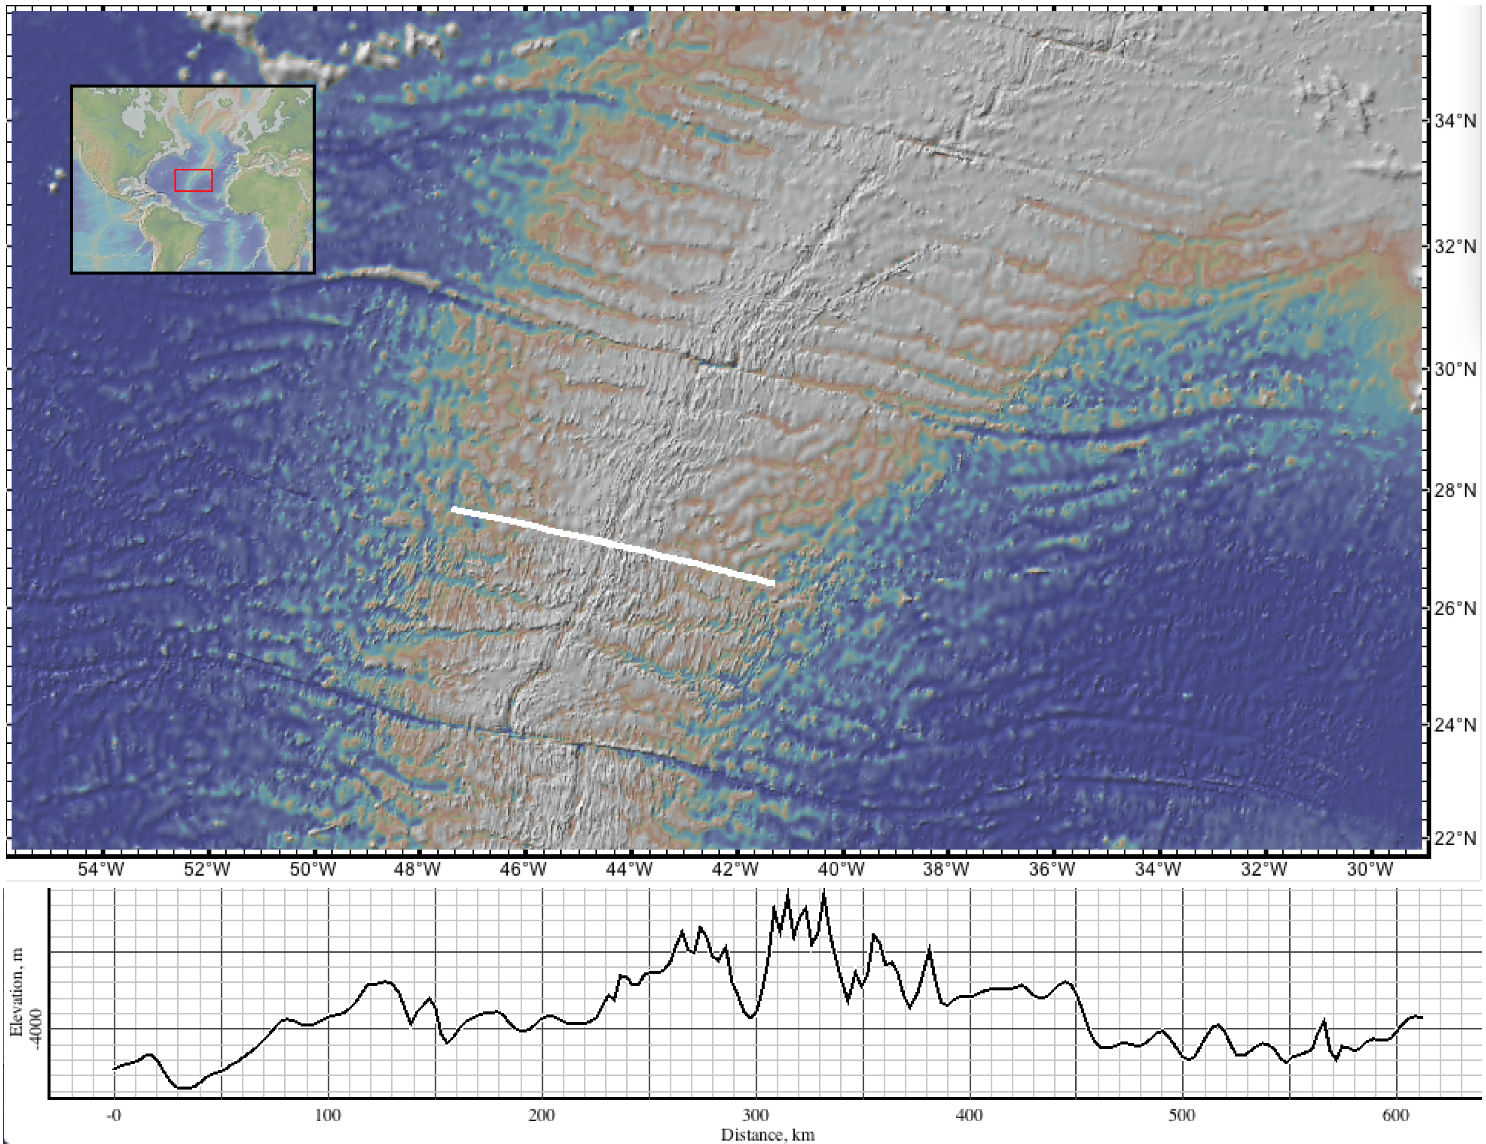
\includegraphics[width=.8\linewidth]{fig1_1.png}
  \caption{\small{Slow spreading Mid-Atlantic Ridge}}
  \label{fig1_1}
\end{subfigure}%
\begin{subfigure}{.5\textwidth}
  \centering
  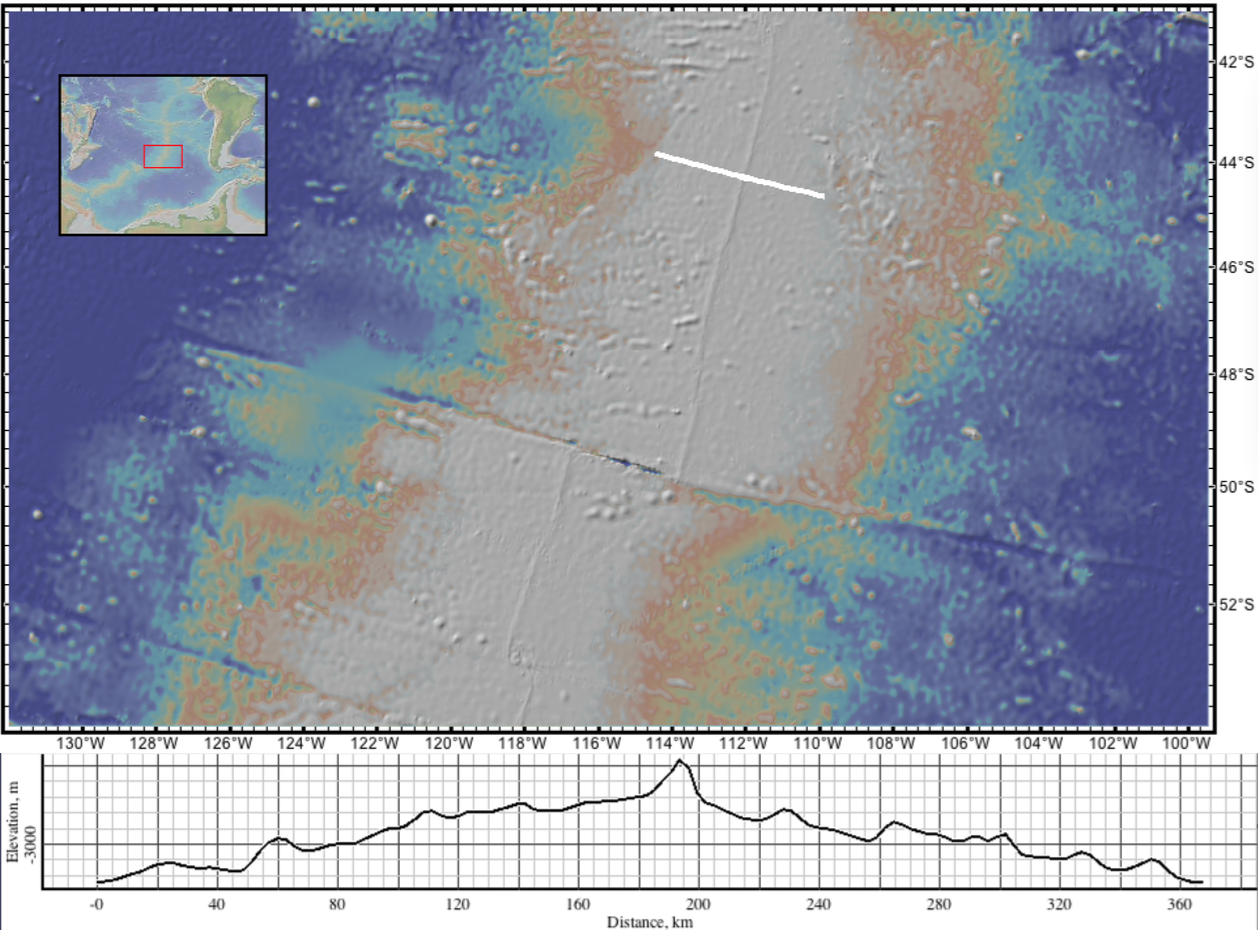
\includegraphics[width=.8\linewidth]{fig1_3.png}
  \caption{\small{Fast spreading East Pacific Rise}}
  \label{fig1_3}
\end{subfigure}
\caption{\small{Topography cross-sections comparison between slow and fast spreading MORs.}}
\label{fig1}
\end{figure}
In addition, slow spreading ridge topography varies distinctly along the ridge axis with respect to the width, depth of the median valleys and the off-axis morphology. As shown by Figure~\ref{fig2_1}, the topography nearer to the center of the ridge segment (A-A') is rather symmetric and has higher frequency with 1km maximum relief while (B-B') is asymmetric and has much lower frequency with 3km maximum relief. Meanwhile, the bathymetry and crust thickness along the ridge valley also varies. From \citep{Chen1999}, the maximum along-axis variation in crustal thickness $\Delta H_{c}$ is linearly increasing with segment length $L$, and the relationship is $\Delta H_{c}(L)=0.0206L$, as shown by Figure~\ref{fig3_1}.

\begin{figure}[H]
 \centering
  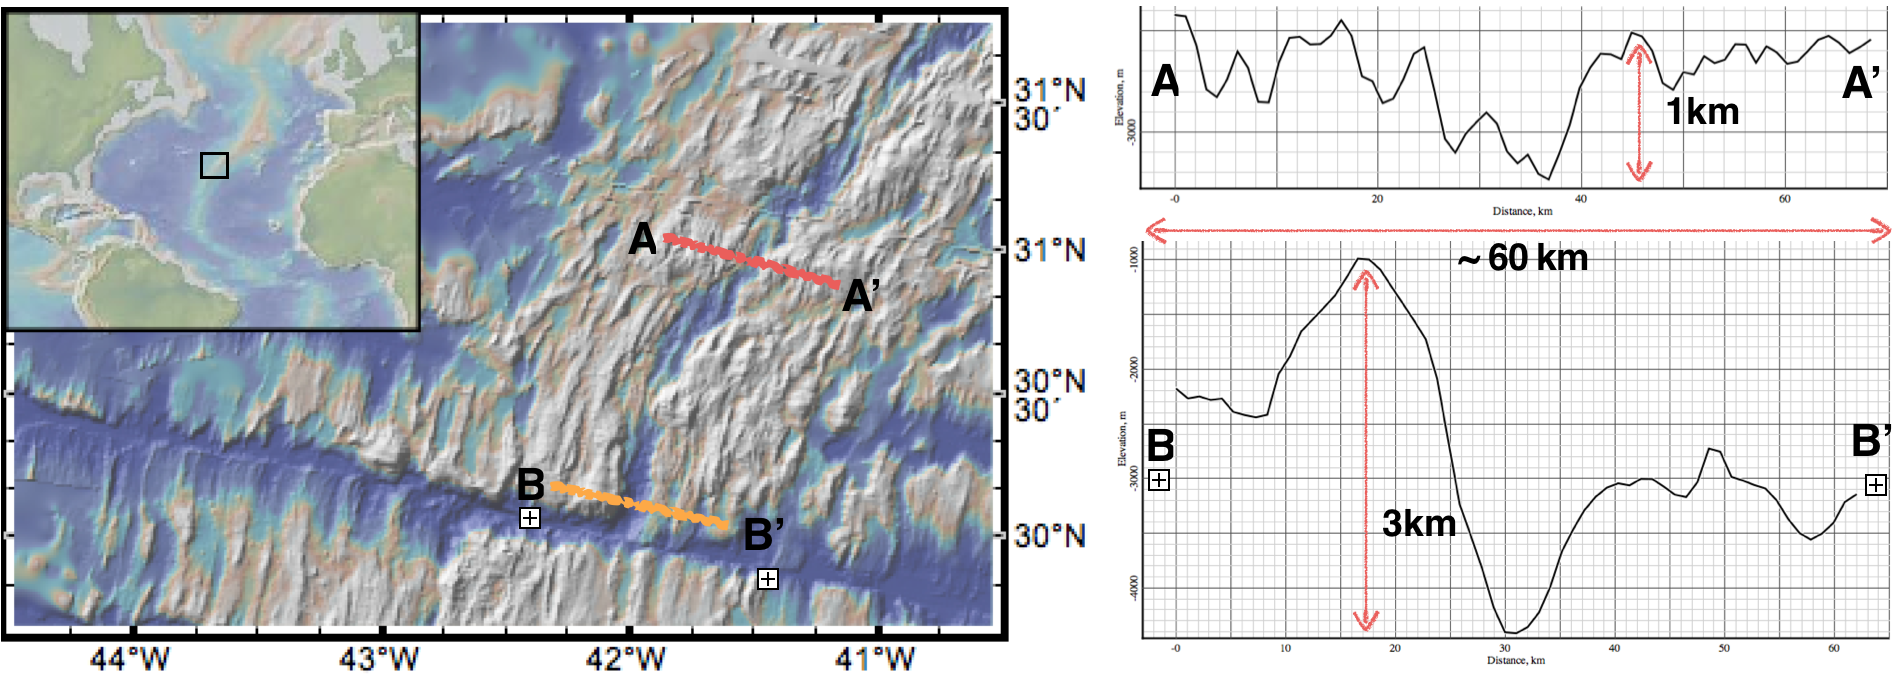
\includegraphics[scale=0.4]{fig2_1.png}
 \caption{\small{Two bathymetry cross-sections of Mid-Atlantic Ridge (MAR) with 10 times vertical exaggeration. A-A' is closer to the ridge segment center while B-B' is at the tip of the segment near the Atlantis Transform fault.}}
 \label{fig2_1}
\end{figure}

\begin{figure}[H]
 \centering
  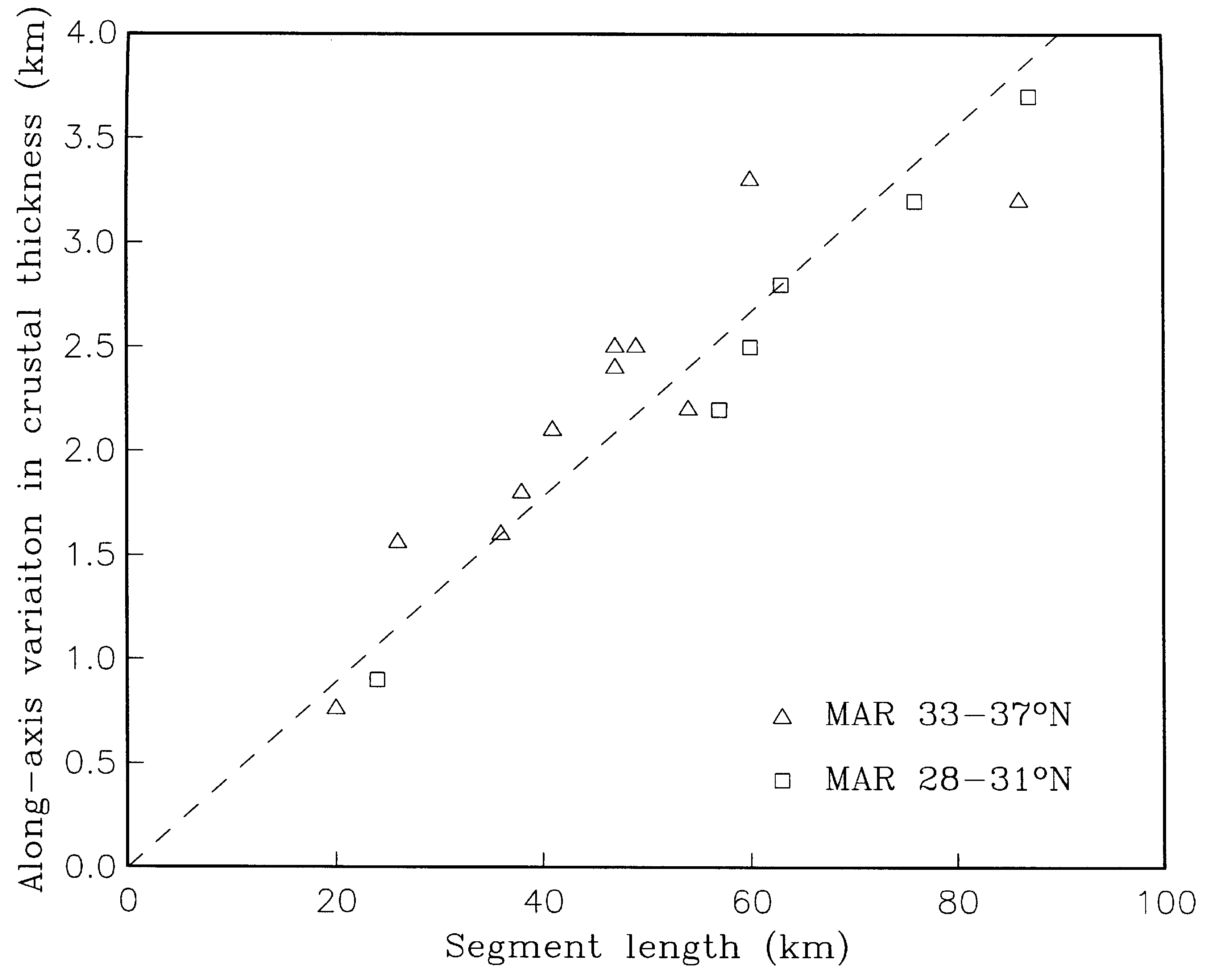
\includegraphics[scale=0.3]{fig3_1.png}
 \caption{\small{Relationship between the maximum crustal thickness variations along a ridge segment and the segment length.The dashed line is the best-fit linear regression of the combined data. \citep{Chen1999}}}
 \label{fig3_1}
\end{figure}

Moreover, a 3D view of B-B' area of Figure~\ref{fig2_1} shows the 20km wide, 25km long and 3km relief Atlantis Massif. The huge geologic structure is a window for learning lower crust and upper mantle because it is believed to be a result of exhumation of deeper material to the seafloor through tectonic processes.

\begin{figure}[H]
 \centering
  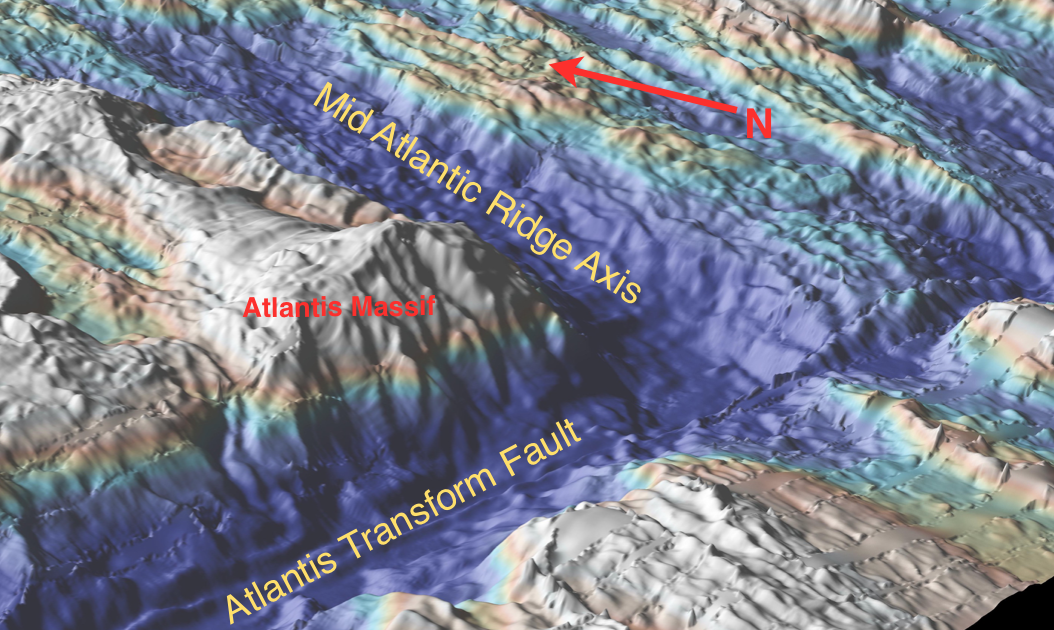
\includegraphics[scale=0.4]{fig4_1.png}
 \caption{\small{Zoom in B-B' area, a 3D view of Atlantis Massif.}}
 \label{fig4_1}
\end{figure}

\subsection{Related work}
\label{ch:related}
As we know, magma supply is mostly a passive process when no hot plume presents \citep{Fowler2004}. Due to vacated room being created by plate separation, decompression will lead to partial melting of the hot mantle beneath the ridges. Then the melt upwells to the surface due to both pressure difference and buoyancy from lateral density difference. When the melt reach the surface with near freezing sea water, it solidifies soon, forming the new crust at the spreading centers and releases the tension from far field stretching. 

The passive nature of magma supply results in the major difference between fast and slow spreading ridges that magma supply is always sufficient to accommodate all the tension built up for fast spreading ridges while is deficit for slow spreading ridges. \citep{Buck2005} explained the distinct difference between fast and slow spreading ridge topography through a 2D modeling study. As shown in Figure~\ref{fig5_1}, for fast spreading ridge, the axial high is generated by buoyancy from lateral density difference across ridge axis and for slow spreading ridge, the median valley is formed due to near-axis normal faulting.
\begin{figure}[H]
 \centering
  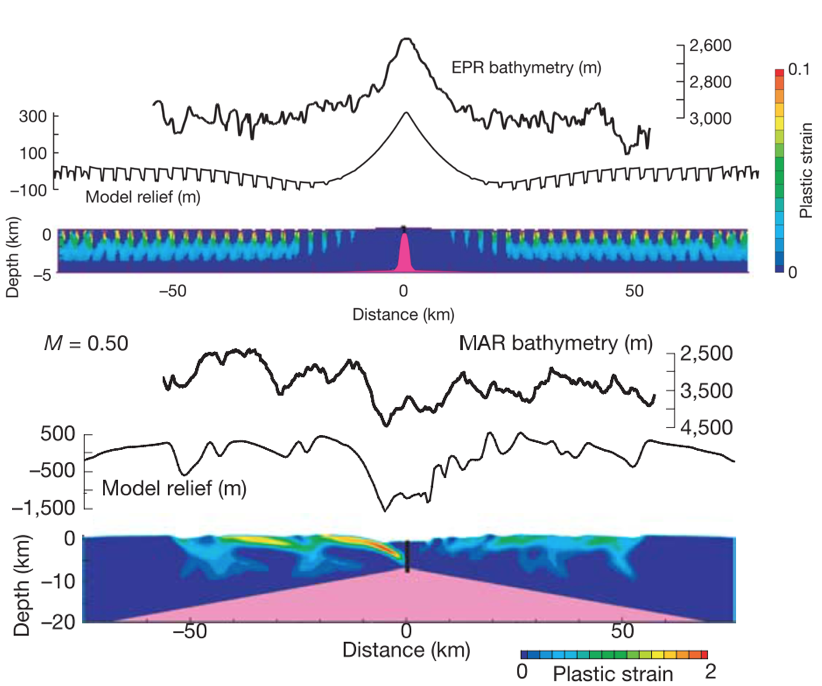
\includegraphics[scale=0.7]{fig5_1.png}
 \caption{\small{Upper one: modeling result for fast spreading agrees well with the observation of East Pacific Rise. Lower one: modeling result for slow spreading ridges agrees well with the bathymetry of Mid Atlantic Ridge. \citep{Buck2005}}}
 \label{fig5_1}
\end{figure}
In addition, a framework of various faulting patterns being controlled by "M" (ratio between rates of magma supply and plate extension) was established. Based on \citep{Buck2005}, \citep{Tucholke2008} moved one step forward. They focus on faulting behaviors of slow spreading ridges and find that the OCCs are most likely to form when M varies from 0.3 to 0.5. As shown in Figure 6, when M=0.7, the fault will be pushed away from axis and is taken place by a new near axis fault when the energy for breaking the new fault becomes less than maintaining the existing one; when M=0.3$\sim$0.5, the normal faults exist for a long time (detachment faults) and the lower crust and mantle material will exhume through the detachment faults and exposed to the seafloor; when M further decreases, most of the tension is accommodated by tectonic process and faulting pattern is more dynamic.
\begin{figure}[H]
\floatbox[{\capbeside\thisfloatsetup{capbesideposition={right,bottom},capbesidewidth=5cm}}]{figure}[\FBwidth]
{\caption{\small A$\sim$F: Faulting behavior for different values of M. Geologic interpretation is superimposed on modeled distribution of strain rate. Dots show breakaways of initial faults. Dashed seafloor is original model seafloor, red dotted seafloor is formed dominantly by magmatic accretion, and solid bold is fault surface. Note that detachment faults in B and C are not interrupted by secondary faults. \citep{Tucholke2008}}}
 {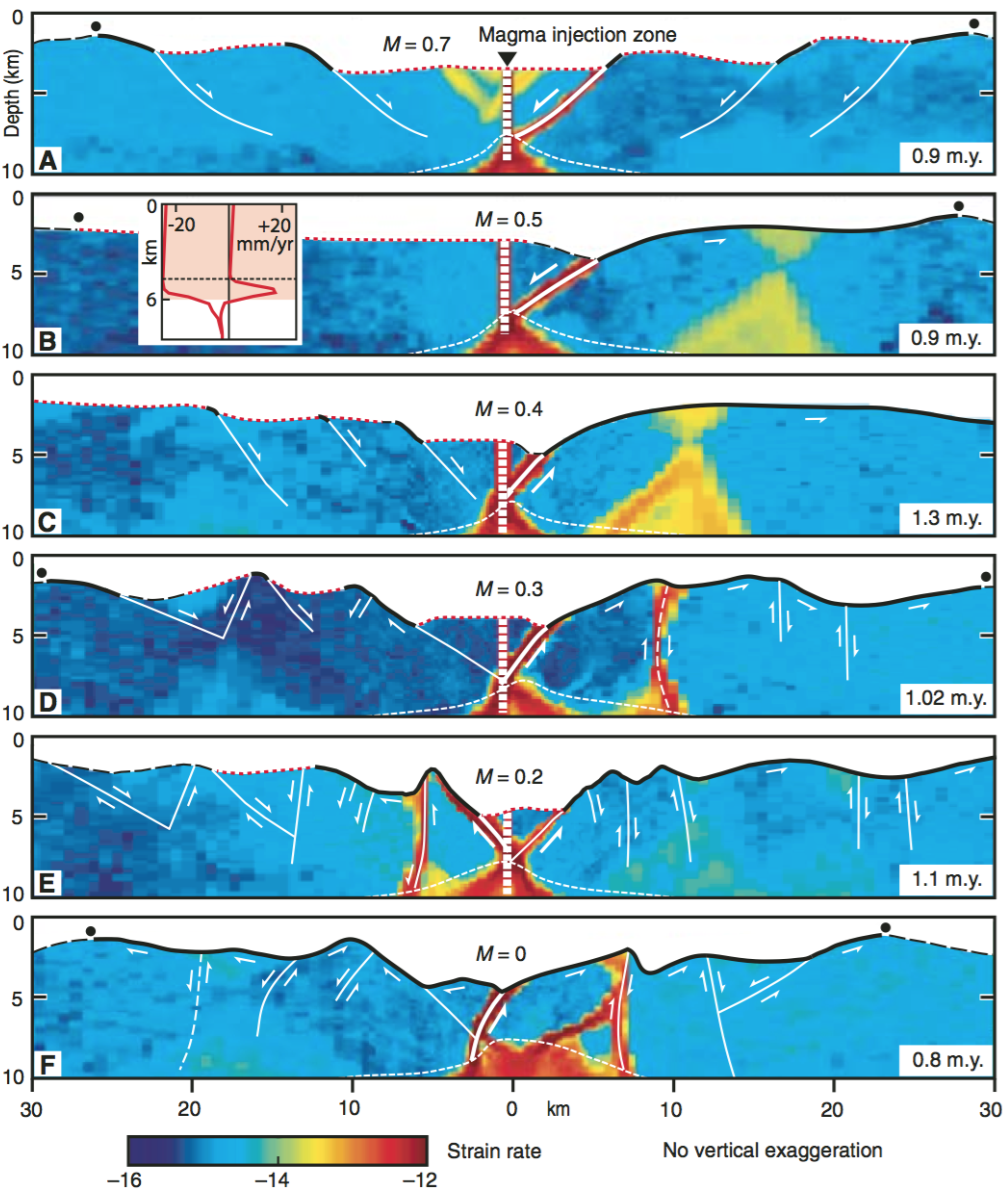
\includegraphics[width=10cm]{fig6_1.png}} 
 \label{fig6_1}
\end{figure}
The "M-factor" framework of the 2D models is successful in explaining various observation of seafloor bathymetry across ridge axis. However, especially for slow-to-intermediate spreading ridges, the interactions between tectonics and magmatism at MORs are inevitably 3D processes (both across and along the ridge axis).

\break
\section{Purpose}
\label{ch:purpose}
As we know, around 70\% of the Earth's crust is oceanic crust and MORs are the most dynamic places where new crust are forming with great amount of earthquakes, volcanic processes constantly happening. To study how new crust is created and how MORs evolve is significant for Earth Sciences. Geodynamics modeling along with a variety of geological, geophysical observation and lab experiment constraints can be used to study how MORs system works under geological time scale of Million years which is impossible to be observed in the length of human history.

Previous studies have established sound framework for tackling the questions. However, 2D models have limitations in studying the along ridge-axis interactions, especially when important variables are not constant along the ridge axis. The passive nature for magma supply results in a constantly sufficient and negligible variation in magma supply along fast spreading ridge axis. The topography along fast spreading ridges does not vary much. However, along the slow spreading ridges axis, controlling variables varies. Bathymetry, gravity anomaly, reflection and refraction seismology consistently show distinguishable variation in crustal thickness \citep{Ryan2009}; \citep{Chen1999}; \citep{Lin1990}; \citep{Tolstoy1993}. Assuming oceanic crust is mainly formed by upwelled magma at the ridge, volume and thus thickness of the crust is a function of magma supply.

Admittedly, at slow spreading ridges, other controlling variables such as hydrothermal cooling, thermal structures and even local spreading rate \citep{Baines2008} also varies both along and across the ridge axis and they are interrelated. But, we propose that the interaction between magmatism and tectonics which is quantified as the ratio "M" is the first order control over the topography evolution of MORs. 

Thus, the purpose of this thesis is to study how the along ridge axis varying "M" will make a contribution to the observed various topography. We will implement the 2D framework "M" into a 3D numerical modeling code SNAC \citep{Choi2008} and focus on the last two questions mentioned in the introduction. Hopefully, through this study, we can explain many fascinating observations along the MORs.

\break
\section{Method of Approach}
\label{ch:method}

The idea is that we utilize geophysical observations and published results to constrain the setups of the 3D model. By iteratively minimizing the gap between results from models and observations, hopefully, a model with consistent results will be generated. Then, we will interpret the observations based on that model.

The numerical modeling code, SNAC, is an explicit Lagrangian finite element code. It is a reusable set of libraries or classes for a software system. It uses the energy-based finite element method to solve the force balance equation for elasto-visco-plastic materials. Figure~\ref{fig7_1} shows major parts of the methods.

\begin{figure}[H]
 \centering
  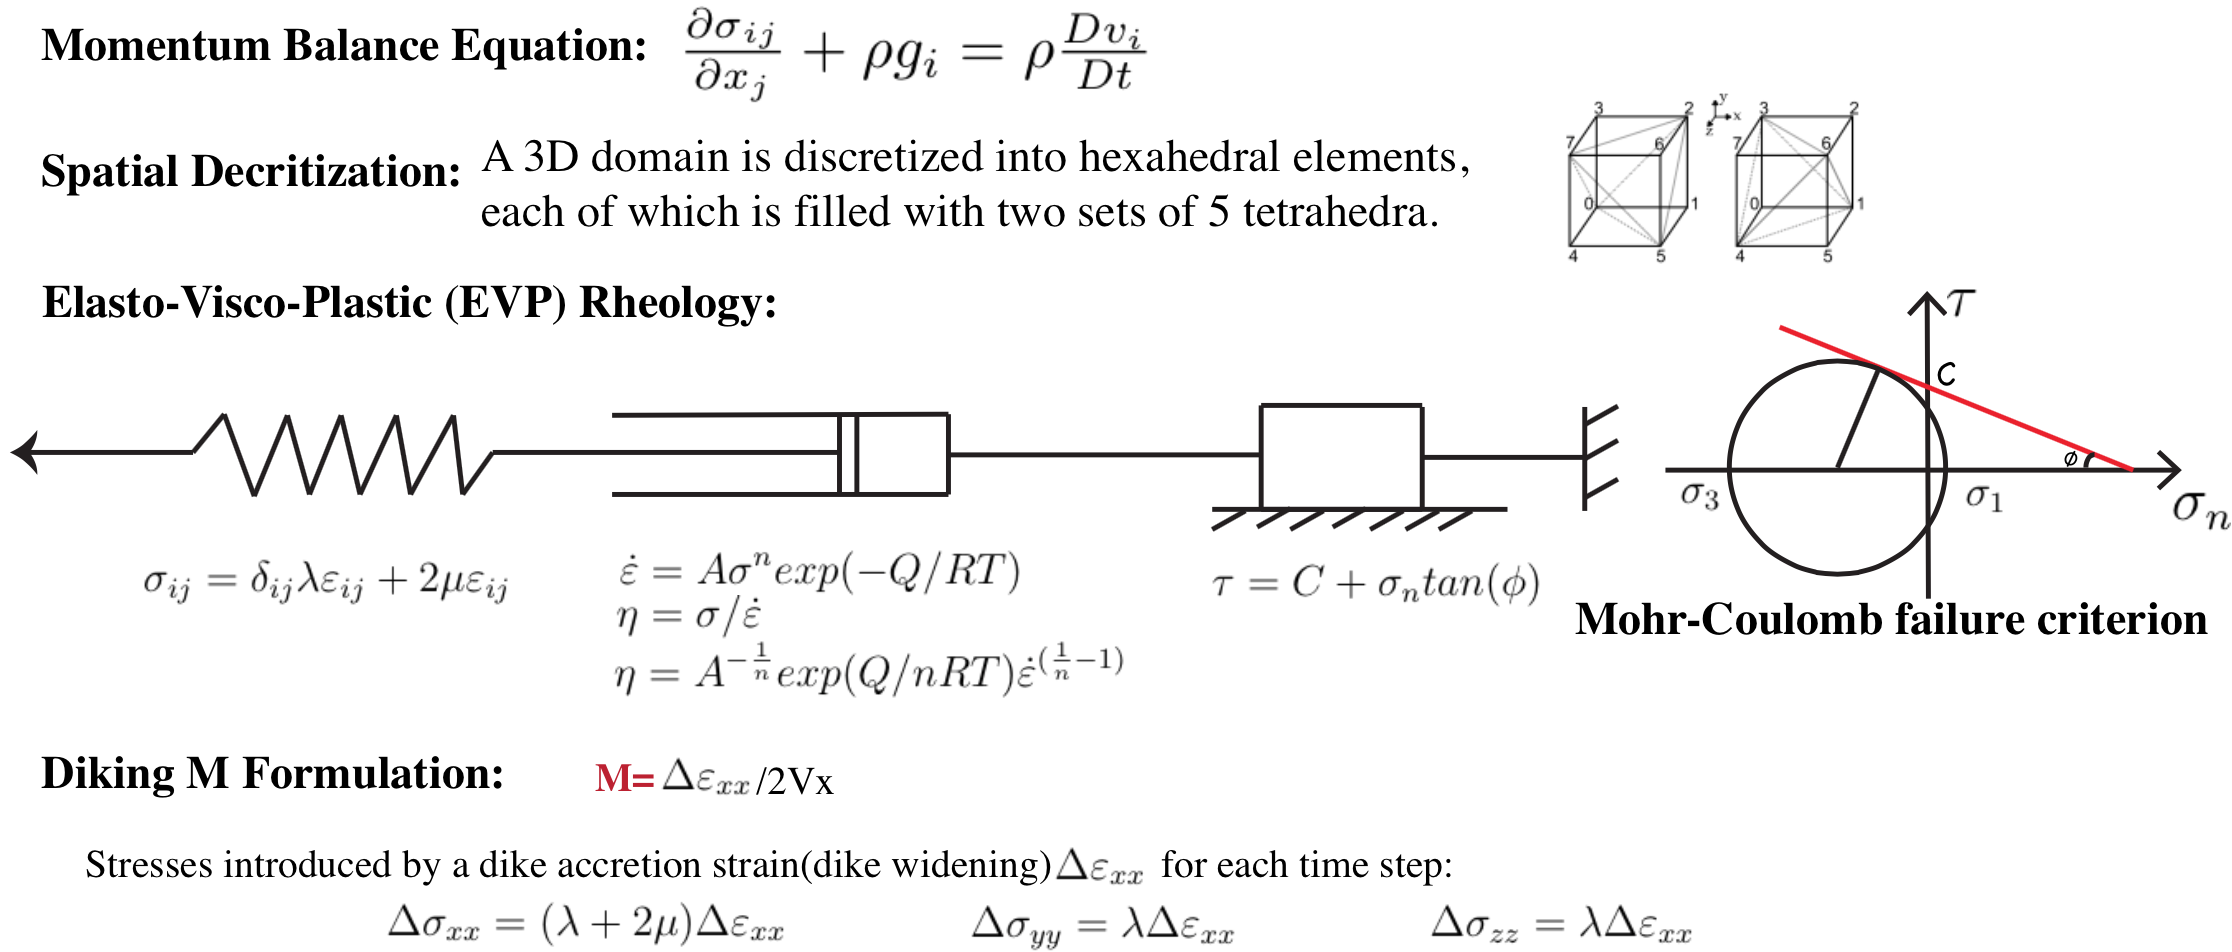
\includegraphics[scale=0.46]{fig7_1.png}
 \caption{\small{Essential theories for the numerical methods}}
 \label{fig7_1}
\end{figure}
 
A number of trial models will be run to find suitable model settings such as thermal and kinematic initial and boundary conditions, viscosity structure and material properties. Preliminary setup is shown in Figure~\ref{fig8_1}. For temperature structure, depth from 0$\sim$6km, linear increases from 0 \degree C to 240 \degree C (remain low for rough approximation of hydrothermal circulation); depth from 6$\sim$20km, instantaneous cooling of a Semi-infinite Half-space (erf function) \citep{Turcotte2002}. For rheology, we will follow dry diabase power law rheology from lab experiments \citep{Kirby1987}. For boundary conditions, free slip on all boundaries, surface temperature is 0\degree C, bottom temperature is 1300 \degree C.


\begin{figure}[H]
 \centering
  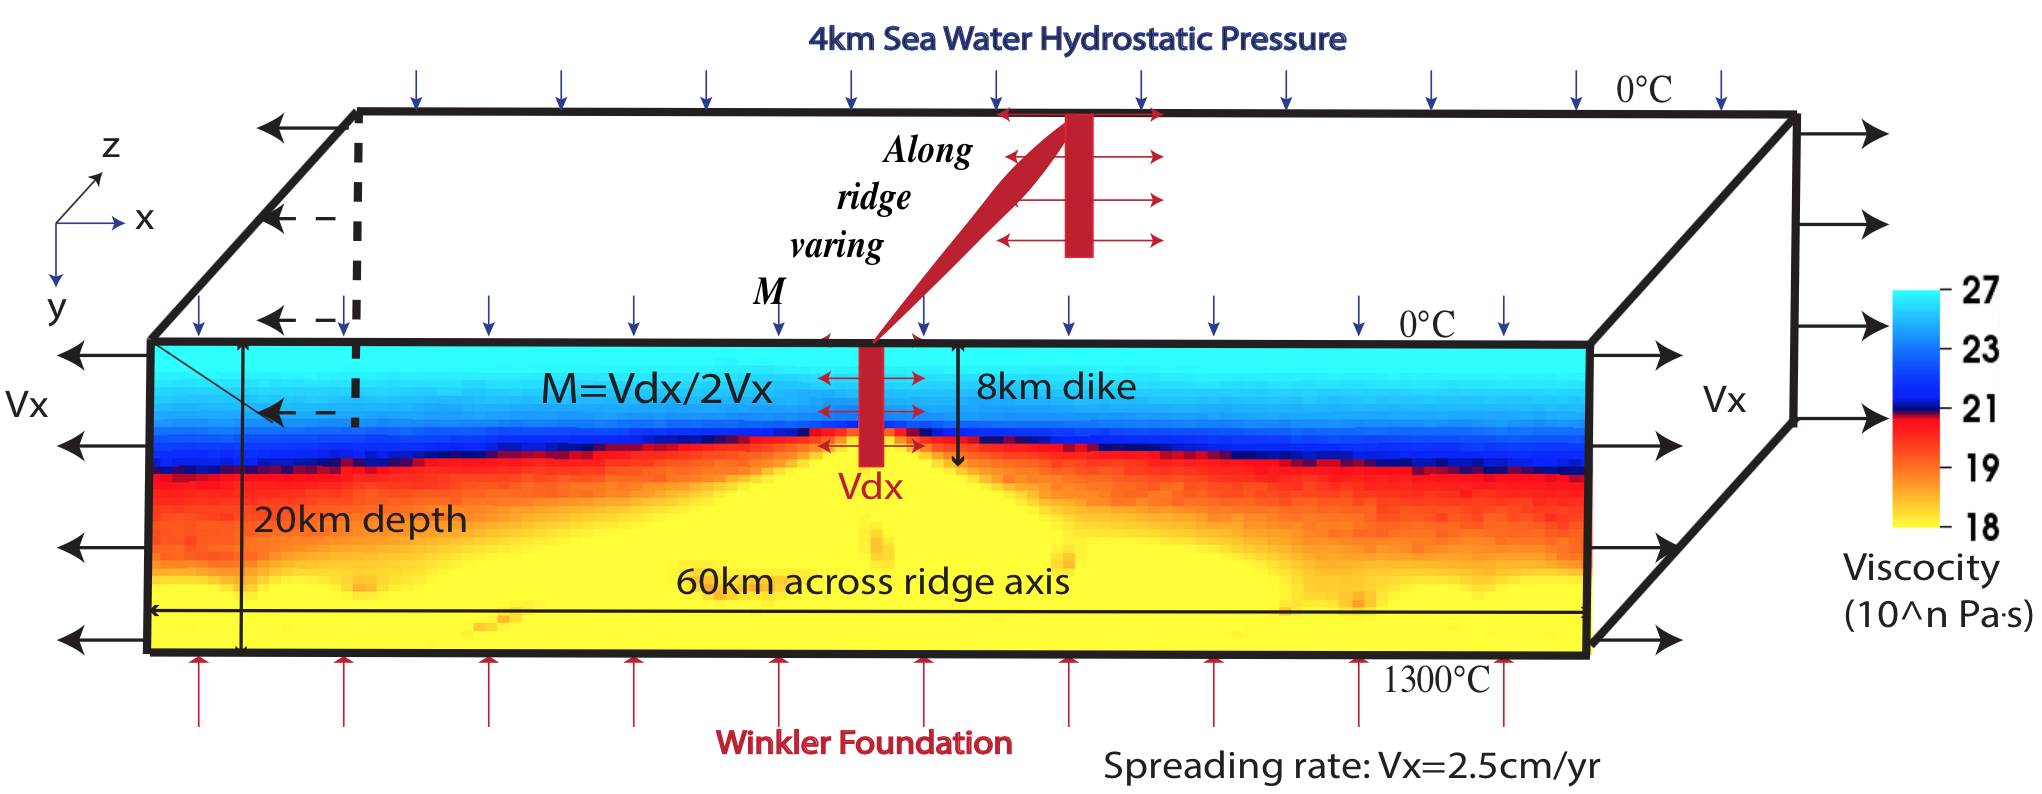
\includegraphics[scale=0.5]{fig8_1.png}
 \caption{\small Preliminary model setup}
 \label{fig8_1}
\end{figure}


Although how the "M" varies along the ridge is not clear due to the complexity of the system and the difficulties of observation (timewise, extremely long geological timescale and spacialwise, deep under the sea water burying under the ridge), we do have constraints from indirect observations (gravity, seismology, geological drilling). Generally, at slow spreading ridges, magma supply mostly at the center of the ridge segment and decreases from the center to the end of the segment \citep{Tolstoy1993}; \citep{Chen1999}. There is also evidence for shorter wavelength of 10 to 20 km discrete focus of magma accretion along the ridge axis \citep{Lin1990}. Based on these constraints, we will test different scenarios of varying "M" along the ridge axis.



\break
\section{Preliminary Results}
First, the formation of Atlantis Massif can be explained by three hypotheses: 
1) For lower M side (front in the model), the long detachment fault (LDF) initiates earlier and then propagates toward higher M side. Lower M means less tension stress will be released by magma supply and thus lead to higher offsetting rate of LDF, which will lead to faster bending and rotating of the LDF. As the lower M side LDF bends, the termination of the LDF will move off axis and thus exhuming lower crustal and upper mantle material further away from axis than higher M side with lower LDF offsetting rate and less bending. This behavior reproduces the characteristic shape of Atlantis Massif. However, observations from geophysical surveys of the M variation along ridge might be opposite to this model result. Thus, other hypotheses need to be tested.
2) Pseudo-2D models show that when M is higher than 0.5, take M=0.8 as an example, the LDF will move off the ridge axis because the hanging wall is "pushed" away by excessive diking. Magma supply accommodates 80\% of the extension while the rest will be accommodated by LDF and the offset of the LDF controls the volume of lower crustal and upper mantle material’s exhumation. Because M decreases from a magma-rich segment center to the segment end, the higher M parts will move off the axis and exhume less while the lower M parts will be maintained near the axis and exhume more. Hence the model reproduced the characteristic shape of Atlantis Massif. 
3) Observing closely in GeoMapApp, I realized that starting from northern tip of the Massif, the ridge axis bent eastward. Considering the shear stress created by the active Atlantis transform fault which will "drag" the decoupled hanging wall of the LDF toward the east, termination of the LDF might migrate toward the axis, exhuming more at the tip of the segment. 

Second, the formation of the adjacent brother domes of Kane Megamullions can be explained by models results with two mechanisms: 1) For M$>$0.5, LDF will move away from the axis. It remains active until the energy for breaking another near axis normal fault becomes less than the energy for maintaining the old one. The initial LDF creates the older dome while a new LDF generates the adjacent one. 2) (shown in 3D video:
M=0.5$\sim$0.8 sinusoidally increases with z, type two weakening) For M$>$0.5 in the whole domain of the ridge segment, LDFs form alternatively on each side of the ridge axis. This behavior also results in adjacent brother domes. 

Third, (observed in 3D, M=0.2$\sim$0.8, square root, type one weakening video), high angle normal offset at 13\degree N Mid-Atlantic Ridge is produced by the model. It is formed when the weak LDF interface extends away from the axis and its front tip overlaps with another accumulated shear stress zone. 

Fourth, as shown in the model, the hanging wall at the high M side (M$>$0.5) will move away from the axis while moving toward the axis at the low M side (M$<$0.5). Observed along-ridge oblique topography lows can be explained by shear stress created by opposite moving hanging walls. 

Fifth, mysterious corrugated oceanic core complex surface is generated by the model and might be explained by trans-tension stress created by the elongated and rotated LDF termination which is a result of along-ridge varying M. 

Sixth, a discussion on frequency of normal faulting was made based on results of hundreds of models. It mainly depends on six parameters: 1) weakening parameters; 2) thickness of the brittle layer; 3) slope of the brittle-ductile transition (BDT); 4) M value; 5) dt and spreading rate; 6) grid-size.

\break
\section{Work Plan}
\label{ch:plan}

Table \ref{tab:plan} shows what have been done so far and what still need to be finished for the completion of the research.

\begin{table}[hc]
\begin{small}
\begin{center}
\begin{tabular}{|l|p{7cm}|l|}
\hline
Timeline & Work & Progress\\
\hline
Dec., 2013$\sim$Jan., 2014& Understand the basics of MORs tectonics and magmatism system & completed\\ \hline
Jan., 2014$\sim$March, 2014& run 2D models in FLAC to understand the framework& completed\\ \hline
March, 2014$\sim$May, 2014& Learn C programing and continuum mechanics and understand the 3D code& completed\\ \hline
May, 2014$\sim$July, 2014& Benchmark pseudo 3D code with previous modeling results& completed\\ \hline
July, 2014$\sim$Sept., 2014& Implement varying "M" into 3D code SNAC& completed\\ \hline
Sept., 2014$\sim$Nov., 2014& Run preliminary 3D models and explain the model behaviors& completed\\ \hline
Nov., 2014$\sim$Dec., 2014& Prepare AGU conference poster and presentation& completed\\ \hline

Jan., 2015$\sim$Feb., 2015  & Run different scenarios of M and systematically examine how M affect the topography & ongoing\\ \hline
Feb. 2015$\sim$March, 2015 & Thesis writting & \\ \hline
April. 2015 & Thesis defense & \\ \hline
\end{tabular}
\end{center}
\end{small}
\caption{An overview of what have been done and plan for what need to be done}
\label{tab:plan}
\end{table}

\pagebreak
\section{Budget}
\label{ch:budget}
Since observations(topography data of mid-ocean ridges) are handy from GeoMapApp, we don’t need to conduct side scan sonar survey in the deep ocean. GeoMapApp can provide very good bathymetry data and images for this research topic. The software as well as the data are free. We might need some other geophysical evidence (seismology, gravity, resistivity, magnetic etc.) to further support results of the model. They can be attained from other people’s research results. Most of the time will be invested in an iteration process—computer calculations on the 3D model and adjustment on the settings of the model and then calculate again based on previous results. Jobs are run on Super computers Stampede and Penguin. They are our HPC expenses.


\break
\begin{footnotesize}
\bibliographystyle{abbrvnat}
\bibliography{Thesis_Proposal.bib}


\end{footnotesize}

\end{document}